\documentclass[leqno,presentation,usenames,dvipsnames]{beamer}
\DeclareGraphicsExtensions{.eps,.jpg,.png,.tif}
\usepackage{amssymb, amsmath, pdfpages, amsfonts, calc, times, type1cm, latexsym, xcolor, colortbl, hyperref, bookmark}
\usepackage{graphicx}
\usepackage{tabularx}
\usepackage{multirow}
\usepackage{listings}
\usepackage{mathpartir}
\usepackage{xspace}

\usepackage[latin1]{inputenc}
\usepackage[english]{babel}

\usetheme{Szeged}
\usecolortheme{beaver}

\definecolor{websiteGreen}{RGB}{107, 224, 134}
\definecolor{silvery}{RGB}{232, 241, 248}
\definecolor{deepOrange}{RGB}{209, 126, 0}

\definecolor{softTan}{RGB}{240, 240, 223}
\definecolor{deepGreen}{RGB}{87, 149, 115}
\definecolor{lilac}{RGB}{199, 164, 202}
\definecolor{lightOlive}{RGB}{168, 166, 96}
\definecolor{deepOlive}{RGB}{101, 109, 41}

\setbeamercolor*{palette primary}{bg=websiteGreen}
\setbeamercolor*{palette secondary}{bg=white}
\setbeamercolor*{palette tertiary}{bg=silvery}
\setbeamercolor*{palette quaternary}{bg=websiteGreen}

\setbeamercolor{section in head/foot}{fg=deepOrange}
\setbeamerfont{section in head/foot}{series=\bfseries}

\setbeamercolor{titlelike}{parent=palette primary,bg=websiteGreen,fg=white}
\setbeamercolor{frametitle}{parent=palette primary,bg=websiteGreen, fg=white}

\addtobeamertemplate{frametitle}{\vspace*{-0.65\baselineskip}}{}

\graphicspath{ {images/} }

\usepackage[latin1]{inputenc}
\usepackage[english]{babel}
% \usetheme{Darmstadt}
\newcommand{\R}{\mathbb{R}}
\newcommand{\N}{\mathbb{N}}
\newcommand{\overbar}[1]{\mkern1.5mu\overline{\mkern-1.5mu#1\mkern-1.5mu}\mkern1.5mu}
\newcommand{\highlight}[1]{
  \addtolength{\fboxrule}{.2ex}
  \begin{block}{}
    \begin{quote}#1
    \end{quote}
  \end{block}
}

\newtheorem*{conjecture}{Conjecture}
\newtheorem*{proposition}{Proposition}

\title{Pecan: An automated theorem prover}
\author[names]{Zhengyao Lin, Eric Ma, Reed Oei, Yikai Teng, Pavle Vuksanovic \\ Christian Schulz, Mary-Angelica Tursi (Team Leaders) \\ Philipp Hieronymi (Faculty Mentor)}

\institute{University of Illinois at Urbana-Champaign}

\date{}

\titlegraphic{%
\vspace{-2em}        
\includegraphics[width = 0.3\textwidth]{UIUC_logo.png}%
\hspace{.30cm}%
\includegraphics[width = 0.07\textwidth]{igl-logo-small.png}%
\\[3ex]%
Illinois Geometry Lab  \\  Final Presentation \\ December 2021\\[2ex]%
}

\include{Pecan/pecan-lang}

\begin{document}
\frame{\titlepage}

\section{Introduction}

\begin{frame}{Automated Theorem Proving}
    \begin{itemize}
        \item An \emph{automated theorem prover} is a program that takes a statement as input and proves, or disproves it, with no human guidance
            
        \item It is impossible to prove \textbf{all} statements automatically
        
        \item Through clever encodings, we can solve interesting problems using theorem provers
    \end{itemize}
    
    \begin{figure}
        \centering
        \includegraphics[width=0.5\textwidth]{images/pecan-demo-sp2020.png}
        \caption{A Pecan program and its output.}
        \label{fig:pecan-ex}
    \end{figure}
\end{frame}

\begin{frame}[fragile]{Pecan}
\begin{itemize}
    \item \textbf{Pecan} is an automated theorem prover we created
    \item It represents logical statements via B\"uchi automata, a model of computation that can handle infinitely long inputs
    \item Try it online at \url{http://reedoei.com/pecan}!
\end{itemize}
    
\begin{pecan}
successor(x, y) := x < y & forallz. z <= x | y <= z

Theorem ("Addition is commutative.", { 
    forallx,y. x + y = y + x 
}).
\end{pecan}
\end{frame}

% \reed{Maybe keep some of this, I'm thinking of putting in a demo for my part}
% \begin{frame}{Features of Pecan}
%     \begin{itemize}
%         \item A completely automatic theorem proving process for statements expressable with B\"uchi automata.
%         \item Automata-based theorem proving is constructive: we can generate counterexamples of false statements.
%         \item Support for custom numeration systems and \emph{automatic sequences} (sequences that can be calculated by an automaton)
%     \end{itemize}
% \end{frame}

% \section{Examples}
% \begin{frame}[fragile]{The Chicken McNugget Problem}
    
% \begin{quote}
%     What is the greatest number of chicken nuggets that cannot be ordered using only boxes of 6, 9, and 20?
% \end{quote}

% \begin{pecan}
% n is purchasable := existsa,b,c. n =$\ $6*a $\color{red} +$ 9*b $\color{red} +$ 20*c
% largest(n) := n = max { n : !(n is purchasable) }
% \end{pecan}
% \vspace{-1em}
% \begin{figure}
%     \centering
%     \includegraphics[width=\textwidth]{images/largest_not_purchasable.pdf}
%     \caption{The B\"uchi automaton representing \pecaninline{largest(n)}, which accepts $110101_2$ ($43$ in base 10) in least significant digit first representation.}
%     \label{fig:largest_non_purchasable}
% \end{figure}
% \end{frame}

% \begin{frame}[fragile]{The Thue-Morse Word}
%     \begin{itemize}
%         \item $T[n] = 1$ if the binary representation of $n$ has an odd number of $1$'s, and $0$ otherwise.
%         \[
%             T = 01101001100101101001011001101001\ldots
%         \]
        
%         \item $p > 0$ is a \emph{period} of a word $w$ if $w$ is of the form $a_0 a_1 \cdots a_{p-1} a_0 a_1 \cdots a_n$; the smallest period of a word is its \emph{least period}.
        
%     \end{itemize}
    
% \begin{pecan}
% p is period(i,j) := p > 0 &
%     forallk. if i <= k & k < j-p then T[k]=T[k+p]
% Prove that {
%     forallp. if p > 0 then 
%         existsi,j. p = min { m : period(i,j,m) }
% }.
% \end{pecan}
% \end{frame}

\section{Sturmian Words}

\begin{frame}
    \frametitle{Sturmian Words}
    
    \begin{itemize}
        \item Imagine hitting a billiard ball at some angle along the line $y = \alpha x$
        \item When the ball crosses a vertical line, write a 0; for horizontal lines, write a 1
        \item Each $\alpha$ defines a \emph{characteristic Sturmian word}, $C_{\alpha}$
    \end{itemize}
    
\begin{figure}
    \centering
    \includegraphics[width=0.5\textwidth]{images/Fibonacci_word_cutting_sequence.png}
    \caption{The characteristic Sturmian word $C_{1/\phi} = 0100101001\ldots$}
\end{figure}
\end{frame}

\begin{frame}{Theorems about Sturmian Words}
    We have used Pecan to automatically prove many theorems about Sturmian words, including:
    \begin{itemize}
        \item Sturmian words are not eventually periodic.
        \item All Sturmian words contain cubes.
        \item Sturmian words contain palindromes of every length.
        \item Sturmian words contain only finitely many antisquares and antipalindromes.
        \item Every subword of a Sturmian word occurs infinitely often.
        \item The unique special factor of length $n$ is the reverse of the length $n$ prefix of the Sturmian word.
        \item $\vdots$
    \end{itemize}
\end{frame}

\section{Multiplication by $\alpha$}
\begin{frame}{Introduction to Ostrowski Representations}
    One of the objects Pecan can prove theorems about are \textbf{Ostrowski representations} of natural numbers.
    \begin{itemize}
        \item Given an irrational base $\alpha$ and its continued fraction expansion, one can find the denominators $q_i$ of the $i$th continued fraction approximation.
        
        \item With some specific rules, it turns out that a number can be written as a sum of multiples of $q_i$ uniquely, and that is called its Ostrowski-$\alpha$ representation.
        
        \item We deal mostly with quadratic irrationals which have a repeating continued fraction expansion, such as the number shown below.
    \end{itemize}
    $$\frac {\sqrt 5 - 1} 2 = \psi = \frac 1 {1 + \frac 1 {1 + \frac 1 {1+\cdots} } }$$
\end{frame}

\begin{frame}{Multiplication by $\alpha$}
    From here we assume that $\alpha$ is a quadratic irrational.
    \begin{itemize}
        \item Akin to multiplying by $10$ in a decimal number system, numbers written in their Ostrowski-$\alpha$ representations can have properties deduced about their product by $\alpha$.
    
        \item There is a way to recognize the ordering of $\mathbb Z [\alpha]$ (the polynomials in $\alpha$) using Ostrowski-$\alpha$ representations in Pecan.
        
        \item The required automata however scale very quickly in complexity based on the complexity of $\alpha$:
        \begin{itemize}
            \item The simplest automata, used for recognition of order in $\mathbb Z [\psi]$, had 2,134 states, while the next simplest had 218,072 states.
        \end{itemize}
        
        
    \end{itemize}
\end{frame}
    

\section{Fractals}
\begin{frame}{Fractals}
    \begin{itemize}
        \item \textbf{Automatic fractals} are fractals recognizable by an automata (through
        some suitable mapping between words and reals)
        \item Utilizing this,
        we developed an extension to Pecan maps the set of words accepted by
        an automata to a subset in $[0, 1]^n$, and plotted some fractals.
    \end{itemize}
\end{frame}

\begin{frame}{Cantor Sets}

    \begin{itemize}
        \item Automata and Plot of the Cantor set:
    \end{itemize}

    \begin{center}
    \includegraphics[width=2.6cm]{FA20/images/fractals/cantor-automata.png}
    \includegraphics[width=3.9cm]{FA20/images/fractals/cantor3.pdf}\\
    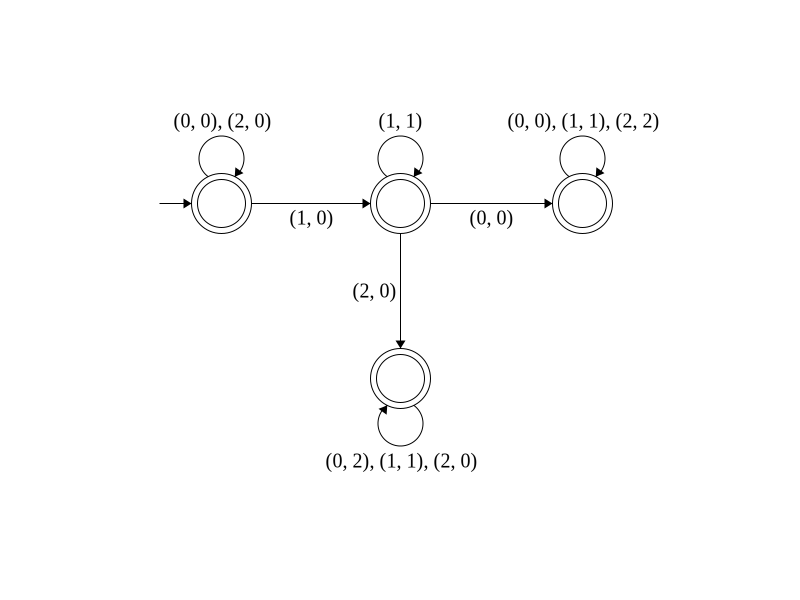
\includegraphics[width=3.9cm]{FA20/images/fractals/cantord-automata.png}
    \includegraphics[width=3.9cm,height=2.6cm]{FA20/images/fractals/cantord.pdf}
    \end{center}
\end{frame}

\begin{frame}{Mooooore Fractals}
    \begin{itemize}
        \item By using a similar automata as the Cantor set, we have the followings:
    \end{itemize}
    
    \begin{center}
    \includegraphics[width=3cm]{FA20/images/fractals/sierpinski-3-l5.pdf}
    \includegraphics[width=3cm]{FA20/images/fractals/sierpinski-5-l3.pdf}
    \includegraphics[width=3cm]{FA20/images/fractals/pascal2.pdf} \\
    \includegraphics[width=3cm]{FA20/images/fractals/menger-3-l4.png}
    \includegraphics[width=3cm]{FA20/images/fractals/vicsek-l5.pdf}
    \includegraphics[width=3.5cm]{FA20/images/fractals/vicsek-3d-l4.png}
\end{center}
\end{frame}

\begin{frame}{Space filling curves}
    \begin{itemize}
        \item By adding a time variable to the automata, we can draw space filling curves like Hilbert curve and Peano curve:
    \end{itemize}
    
    \begin{center}
    \includegraphics[width=2.5cm]{FA20/images/fractals/hilbert-automata.png}
    \includegraphics[width=2.5cm]{FA20/images/fractals/hilbert-1.pdf}
    \includegraphics[width=2.5cm]{FA20/images/fractals/hilbert-2.pdf}
    \includegraphics[width=2.5cm]{FA20/images/fractals/hilbert-1.pdf} \\
    \includegraphics[width=3cm]{FA20/images/fractals/peano-automata.png}
    \includegraphics[width=2.5cm]{FA20/images/fractals/peano-1.pdf}
    \includegraphics[width=2.5cm]{FA20/images/fractals/peano-2.pdf}
    \includegraphics[width=2.5cm]{FA20/images/fractals/peano-3.pdf} \\
\end{center}
\end{frame}

\section{Future Work}
\begin{frame}{Future Work}
    \begin{enumerate}
        \item Continue to develop Pecan.
        \item Explore other extensions to Pecan.
    \end{enumerate}
\end{frame}

\end{document}
